\chapter{Introducing the Emotiv EPOC}
\label{cha:epoc}

\section{SDK description}
The Emotiv EPOC headset is a portable EEG device which consists of 14 sensors that transmit raw EEG data (see figure \ref{fig:sensorPos} for their positioning) to the computer and 2 reference sensors (CMS - Common Mode Sense and DRL - Driven Right Leg). The CMS sensor is the point on the scalp against which everything else is measured. The DRL sensor provides a feedback signal to cancel common mode noise in the electronics \cite{refSensors1, refSensors2}. See table \ref{table:sensorName} for the meaning of the abbreviations of sensor positions. The raw data gets interpreted and the user gains access to all of the information in one of the following 4 suites: Expressiv, Affectiv, Cognitiv, Mouse Emulator. 

\begin{figure}
  \centering
  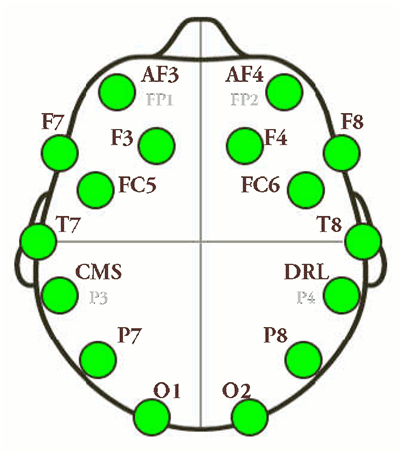
\includegraphics[width=250px]{sensorPositioning.png}
  \caption{Sensor positioning for the Emotiv EPOC. Credit: Emotiv}
    \label{fig:sensorPos}           
\end{figure}

\begin{table}[h]
\centering
\begin{tabular}{|c|c|llcc}
\cline{1-2} \cline{5-6}
\textbf{Abbreviation} & \textbf{Meaning} &  & \multicolumn{1}{l|}{} & \multicolumn{1}{c|}{\textbf{Colour code}}          & \multicolumn{1}{c|}{\textbf{Meaning}} \\ \cline{1-2} \cline{5-6} 
A                     & Ante             &  & \multicolumn{1}{l|}{} & \multicolumn{1}{c|}{Black}                         & \multicolumn{1}{c|}{No signal}        \\ \cline{1-2} \cline{5-6} 
F                     & Frontal          &  & \multicolumn{1}{l|}{} & \multicolumn{1}{c|}{{\color[HTML]{FE0000} Red}}    & \multicolumn{1}{c|}{Very poor signal} \\ \cline{1-2} \cline{5-6} 
C                     & Central          &  & \multicolumn{1}{l|}{} & \multicolumn{1}{c|}{{\color[HTML]{F8A102} Orange}} & \multicolumn{1}{c|}{Poor signal}      \\ \cline{1-2} \cline{5-6} 
P                     & Parietal         &  & \multicolumn{1}{l|}{} & \multicolumn{1}{c|}{{\color[HTML]{F8FF00} Yellow}} & \multicolumn{1}{c|}{Fair signal}      \\ \cline{1-2} \cline{5-6} 
T                     & Temporal         &  & \multicolumn{1}{l|}{} & \multicolumn{1}{c|}{{\color[HTML]{32CB00} Green}}  & \multicolumn{1}{c|}{Good signal}      \\ \cline{1-2} \cline{5-6} 
O                     & Occipital        &  &                       & \multicolumn{1}{l}{}                               & \multicolumn{1}{l}{}                  \\ \cline{1-2}
\end{tabular}
\caption {Left: Abbreviations for sensor positioning; Right: Sensor contact quality and colour codes}
\label{table:sensorName}
\end{table}

I have been using the developer's SDK, so it is worth highlighting I did not have any access to the raw EEG data. 

The battery lasts about 10 to 12 hours. The charging is done via a USB cable.

According to \cite{experimenterEPOC}, the data sampling rate is 128Hz. \cite{emotivUserManual} states that there may be up to 2 seconds delay from when the data is sent until a visual feedback is observed. 

\subsubsection{Expressiv\texttrademark  Suite}
Detects 12 facial expressions:
\begin{multicols}{2}
\begin{enumerate}
	\item Blink
	\item Left wink
	\item Right wink
	\item Look left
	\item Look right
	\item Smile
	\item Laugh
	\item Smirk left
	\item Smirk right
	\item Raise brow
	\item Furrow brow
	\item Clench teeth
\end{enumerate}
\end{multicols}
One thing to note is that if the sensor contact quality is not perfect, blinks and winks might be mistaken; same applies to laughs and smiles. In fact, an ideal signal is obtained when all sensors display green (see table \ref{table:sensorName}). It is acceptable to have some displaying yellow but anything less than yellow, means data might be unreliable or unavailable.
	
The API usually gives back data as a \texttt{boolean}, but for smile, clench and look left/right, a \texttt{float} between 0 and 1 can also be obtained which represents the extent of that facial expression. 

Figure \ref{fig:blinkAF} shows an image of how the EEG looks like in channels AF3 and AF4 after a blink. See figure for a screenshot of the suite.

\begin{figure}
  \centering
  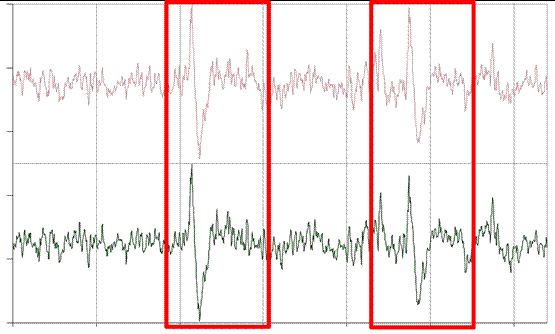
\includegraphics[width=350px]{eyeBlink.png}
  \caption{AF3 and AF4 channel response to eye blink. Credit: \cite{experimenterEPOC}}
    \label{fig:blinkAF}           
\end{figure}

\subsubsection{Affectiv\texttrademark  Suite}
\label{part:affectiv}
Returns a \texttt{float} between 0 and 1 which describes the power of one of the following emotions:
\begin{itemize}
	\item Engagement/Boredom
	\item Frustration
	\item Meditation
	\item Excitement short term
	\item Excitement long term
\end{itemize}

I have found that these emotions represent my mood quite well. One thing to note is that boredom is not the kind of boredom one feels when they have nothing to do, but it is rather the opposite of engagement, according to Emotiv. See figure for a screenshot of the suite.

The Emotiv User Manual \cite{emotivUserManual} (page 31) provides information on the activities and brainwave types that may trigger each emotion.

\subsubsection{Cognitiv\texttrademark  Suite}
This is probably the most exciting feature of the Emotiv EPOC. Here, you can train 13 actions: push, pull, left, right, lift, drop, 6 rotations (one in each direction for the X, Y and Z axis) and disappear. The disappear action is more abstract because while the first 12 are real life actions, an object cannot vanish into thin air, in reality, through whatever methods. The user has to train each action for a period of 8 seconds. This should be done multiple times until an as high as possible skill level is obtained. The more you get used to training, the easier it will become. I have achieved close to 100\% on all 4 actions: push, pull, left, right. At one point, I was able to achieve 100\% on the push action in less than 5 trainings. The SDK can only detect up to 4 actions at any one time, so one has to choose wisely which actions would be best for their application. See figure \ref{fig:skillLevelMe} for a screenshot of the suite.

\subsubsection{Mouse Emulator (Gyro)}

This data actually comes from a gyroscope fitted in the headset. The original version aims to emulate the mouse movement by changing the head position. Once your head turns to left or right and remains in that position, the centre of the circle becomes your new head position. However, I had access to the Unity 3D plugins and I was able to modify this suite so that the centre of the circle was not recalculated if the head stayed to the left or to the right because I wanted to use the gyro as yet another way to control the car movement. See figure for a screenshot of the suite.

\subsection{Caring for the headset}
The 16 sensors need to be properly hydrated before starting to use the Emotiv EPOC. The hydration is done with contact lenses saline solution which has the purpose of enabling a better transmission of the brainwaves while also sanitising the felt pads. For the first use of the sensors, one may need to apply 15-20 proper hydrations before good and reliable sensor contact quality is achieved.

When the user does not expect to use the headset for a period of more than 3-4 days, it is recommended to remove the felt parts from the sensors. Otherwise, the process of oxidation happens much more quickly. See figure \ref{fig:cleanVsOxidised} for images of clean sensors and oxidised sensors. The green residue can be cleaned with a cotton swab dipped into a solution of 1/2 water 1/2 white vinegar. If cleaning the interior of the golden plates, take care not to remove the slightly white polymer paste. I have left the felt parts in the sensors when I went on holiday for about 3 weeks. When I returned, the headset was losing contact quality very quickly and after about 15 minutes, it had to be rehydrated. It looks like salt columns may also form in the felt parts. My problem though, was that the golden plates oxidised a lot and after cleaning them as described above I achieved full green sensor contact quality which is the best you can wish for. I firstly cleaned the outside of the golden plates but that did not help too much. Then, I moved to cleaning the inside as well and that did the job for me, although on the Emotiv forums this is not something they would recommend. I was amazed to see the great contact quality I could achieve and it did not have any negative effects on the sensors as they are still in perfect shape 3 months after the cleaning.

\begin{figure}
  \centering
  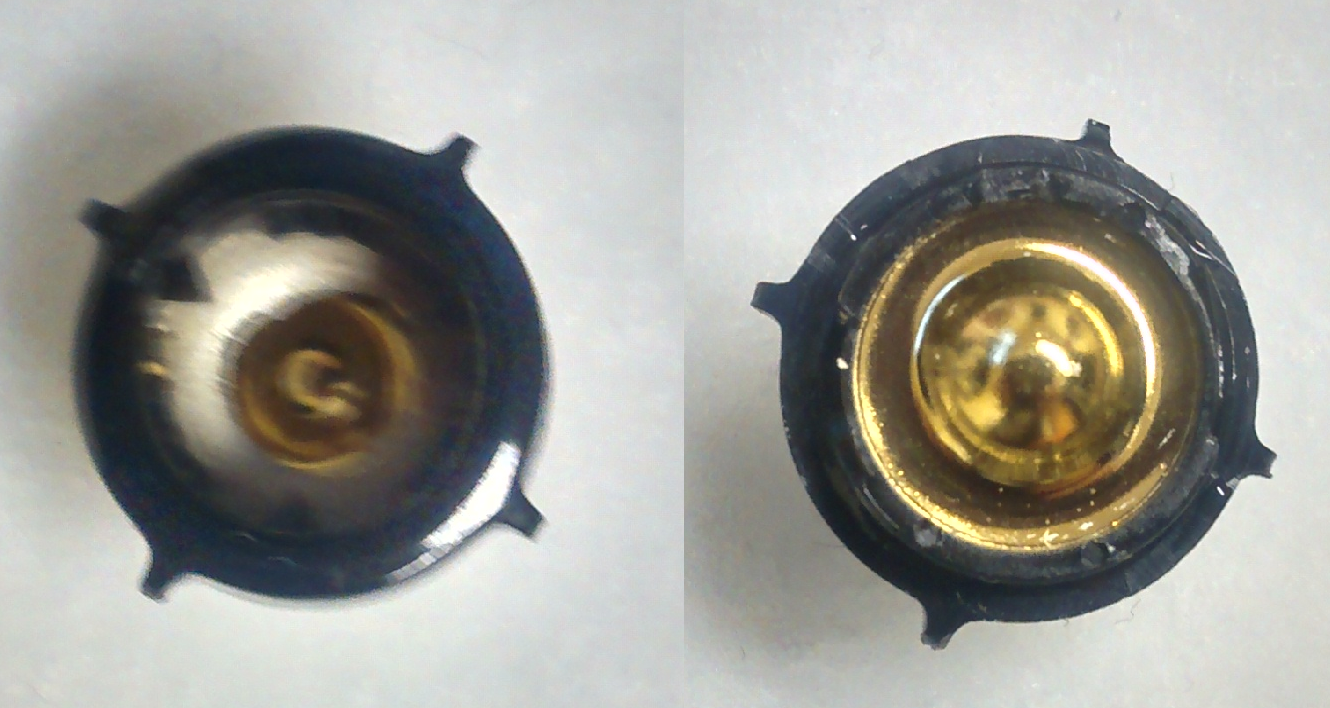
\includegraphics[width=350px]{goodSensorBadSensor.png}
  \caption{From left to right: clean inside of golden plate; clean outside of golden plate; oxidised inside of golden plate; oxidised outside of golden plate.}
    \label{fig:cleanVsOxidised}           
\end{figure}

\subsection{Headset issues}
One of the main problems I encountered is that the wireless connection to the computer is not reliable and it can drop out of the blue. The EPOC+ is now on the market and it seems it might come with a solution for this.

\subsection{EmoComposer}
\label{part:emocomposer}
EmoComposer is a tool which sends simulations of EmoEngine events to an application. This made it easy to test my game without connecting the headset. This was particularly useful in more tricky to test situations which would have meant spending a long time trying to achieve an action by pure concentration.

\subsection{EmoKey}
EmoKey allows mapping of keys to all the interpretations described in this chapter. In this way, one can use the headset to send smiley faces when smiling or laughing for example. One may also use it to paint. These are two of the things that I have tried. It is supposed to be more useful for playing games using the headset. This has been tried in \cite{wowControl} for the \textit{World of Warcraft} game.

\section{Training}
Because training is a difficult part of getting started with the headset, this section is only trying to provide some pointers as to what might work. 

First of all, while training the user should try to keep as still as possible and concentrate on the action being trained. For example, if one is trying to train the push action, the thing which works most of the times is to visualise how the training cube is being pushed to the back of the virtual room. 

Other people find it easy to visualise a flow of energy in the direction of the trained action. 

Repeating words into one's mind does not work. I have seen it working when people say words out loud but the same pace should be kept.

Doing hand gestures works sometimes as \cite{emoTraining} seems to suggest. I have seen one user trying to do this. It worked for a while but then it stopped. Same happened to me.

One thing I have not tried is shifting concentration on the left or right hand side of the body as it iss suggested in \cite{emoTraining}.

Imagining colours or objects for different actions, does not seem to work.

The problem with training is that there is no `recipe' one can follow. Rather, the user has to try to come up with something that works for them. 

With regards to the training success, in figure \ref{fig:skillLevelMe} you can see one of my achievements. \cite{emoTraining} suggests the fastest learners seem to be young children who believe they can do anything, and very relaxed elderly. In the given example, the father of the poster, aged 82, was able to train reliably 4 actions in less than 5 minutes. For some notes on how my user testing training worked, read chapter \ref{cha:testing}.

\begin{figure}
  \centering
  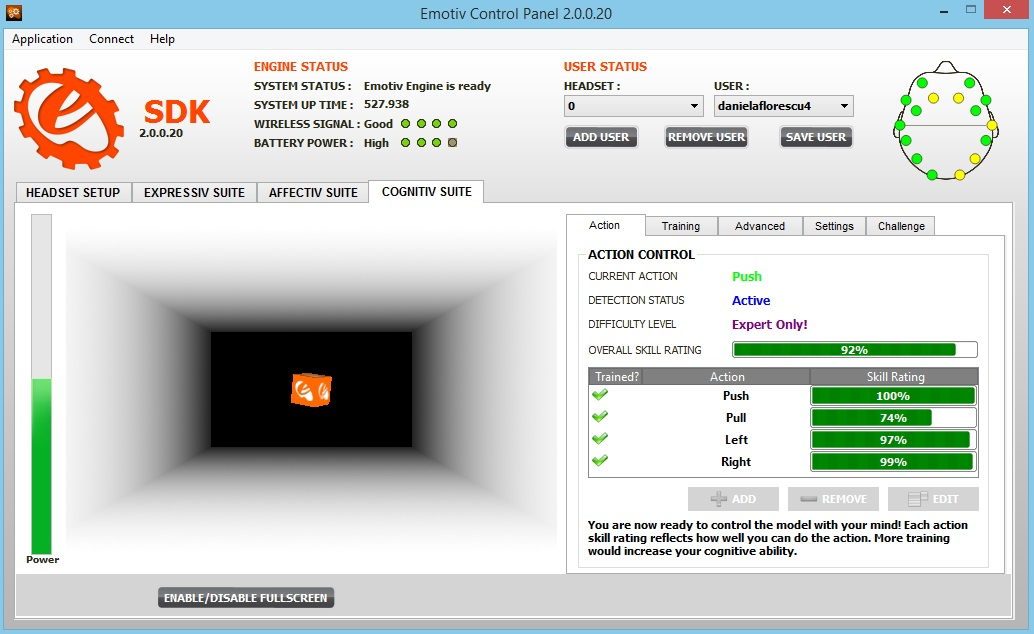
\includegraphics[width=400px]{skillLevel.png}
  \caption{Cognitiv suite training profile}
    \label{fig:skillLevelMe}          
\end{figure}

Some people might encounter difficulties in training the headset. According to \cite{cureBCIilliteracy}, between 15\% and 30\% of the people trying to use a BCI, will not be able to do so. This condition is called `BCI illiteracy' and it better analysed by \cite{BCIilliteracy}. Their study suggests these people have high theta and low alpha waves present across different mental states such as non task related, resting before motor imagery and motor imagery. \cite{cureBCIilliteracy} have tried to come with a solution to this by using a subject-optimised classifier.

\section{Current Applications}
In this section, I am going to have a quick go-through some of the existent applications developed with the help of the Emotiv EPOC.

\begin{itemize}
	\item NeuroPhone \cite{neurophone} is an application which uses the P300 signal and allows the user to scroll through photos of 6 contacts at a time. Once the person the user is looking for is found, the application will dial that person's number.
	\item \cite{handOrthotic} have developed a system which allows the control of a hand prosthetic which opens and closes a patient's hand.
	\item \cite{wheelchairEEG} shows it is difficult to successfully control applications in a highly error sensitive context, such as a wheelchair. 
	\item Mindtunes \cite{mindtunes} is a project in which DJ Fresh has used multiple headsets in order to produce club quality music from the raw EEG data.   
	\item EmoLens \cite{emoLens} tags a user's Flickr photos with emotions and learns to show similar pictures in the future as well as allowing picture search based on the tagged emotion.
\end{itemize}